\documentclass[11pt, A4paper, norsk]{article}
\usepackage[utf8]{inputenc}
\usepackage[T1]{fontenc}
\usepackage{babel}
\usepackage{amsmath}
\usepackage{amsfonts}
\usepackage{amsthm}
\usepackage{amssymb}
\usepackage[colorlinks]{hyperref}
\usepackage{listings}
\usepackage{color}
\usepackage{hyperref}
\usepackage{graphicx}
\usepackage{cite}
\usepackage{textcomp}
\usepackage{float}
\usepackage{color}

\definecolor{url}{rgb}{0.1, 0.1, 0.4}
\graphicspath{{/home/torstein/Dokumenter/UiO/Utveksling/}}
\hypersetup{colorlinks, urlcolor=url}

%\includegraphics[width=12.6cm, height=8cm]{<Filnavn type png>}
%To crop a picture insert 
%trim={<left> <lower> <right> <upper>}, clip
%as kwargs

\hypersetup{colorlinks, urlcolor=url}



\begin{document}
I was not able to take a specific test within the timelimit i was given. Still I hope this information given is enought to lett me take an excange semester in your university. \\
The English language is one of the official languages used for our exam, and lectures are held in english if not all students understand norwegian. \\
I have taken 2 courses which gives lectures in English as it is normal for nonnorwegian students to take these courses. \\
FYS3140 : \url{https://www.uio.no/studier/emner/matnat/fys/FYS3140/index-eng.html} \\
FYS2160 : \url{https://www.uio.no/studier/emner/matnat/fys/FYS2160/index-eng.html} \\
AST2210 : \url{https://www.uio.no/studier/emner/matnat/astro/AST2210/index-eng.html}

I will also include a picture of my diploma from my high school where I had two years of English education. This is of cource after the mandetory 9 years of English education from the age of 7 to 16. For information the grade system in Norway is from 1 to 6 where 3 is the average grade among students. \\
In the picture below you can see the obligatory class English(called Engelsk in norwegian) with the grade 4, and the voulentary classes International English writing(Internasj. engelsk, skriftlig) and International English oral(Internasjonal engelsk, muntlig) with the grades 5, 5 and 4. \\
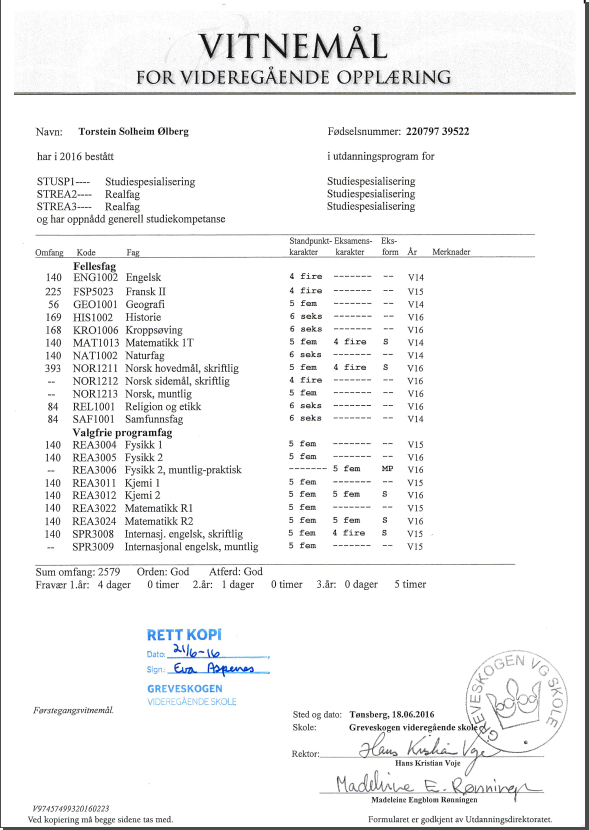
\includegraphics[width=400pt, height=550pt]{Vitnemal.png}
\end{document}